\iffalse
\documentclass[journal,12pt,twocolumn]{IEEEtran}
\usepackage{amsmath,amssymb,amsfonts,amsthm}
\usepackage{txfonts}
\usepackage{tkz-euclide}
\usepackage{listings}
\usepackage{gvv}
\usepackage[latin1]{inputenc}
\usepackage{adjustbox}
\usepackage{array}
\usepackage{tabularx}
\usepackage{pgf}
\usepackage{lmodern}
\usepackage{circuitikz}
\usepackage{tikz}
\usepackage{graphicx}
\begin{document}
\bibliographystyle{IEEEtran}

\vspace{3cm}

\title{}
\author{EE23BTECH11047 - Deepakreddy P
}
\maketitle
\newpage
\bigskip


\noindent \textbf{3} \quad A 44 mH inductor is connected to 220 V, 50 Hz ac supply. Determine
the rms value of the current in the circuit.\\
\solution
\fi


\begin{figure}[ht]
  \centering
      \begin{circuitikz}[american]
   \draw (0,0) to [L=44mH](0,3) to (3,3)[short] to [sV=220V](3,0) to [short](0,0);
\end{circuitikz}

  \caption{Circuit-1}
\end{figure}

\begin{align}
    V &= I \brak{j \omega L} \\
    I &= \frac{V}{j \omega L} A \\
    I &= \frac{220 \sqrt{2}}{j \brak{314} \brak{44 \text{x} 10^{-3}}}A\\
    I &= \frac{22.52}{j}A
\end{align}


\begin{figure}[ht]
  \centering

      \begin{circuitikz}[american]
   \draw (0,0) to [L=$44j\omega $](0,3) to (3,3)[short] to [sV=220V](3,0) to [short](0,0);
\end{circuitikz}


  \caption{Circuit-2}
\end{figure}

\begin{align}
    I_{rms} = \frac{I}{\sqrt{2}}A\\
    I_{rms} = \frac{15.92}{j}A\\
    \abs{I_{rms}} = 15.92 A
\end{align}

\begin{figure}[ht]
   \centering
   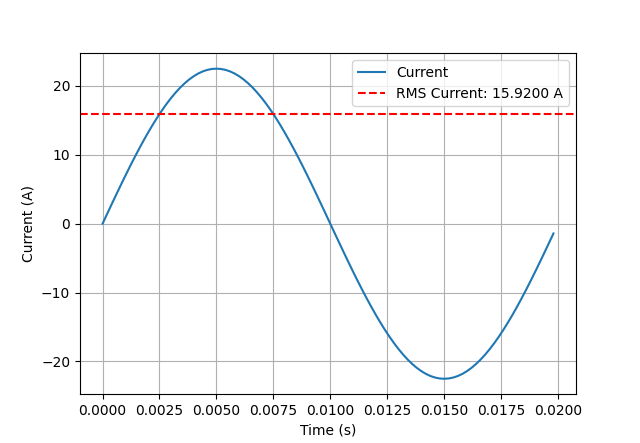
\includegraphics[width=1.1\columnwidth]{ncert-physics/12/7/3/figs/ac.png}
   \caption{Plot of I vs time}
\end{figure}

\begin{center}
    \begin{table}[ht]
        \setlength{\arrayrulewidth}{0.3mm}
\setlength{\tabcolsep}{12pt}
\renewcommand{\arraystretch}{1.3}


\begin{center}
\caption{Input Parameters}
\begin{tabular}{ |p{1.7cm}|p{1.7cm}|p{1.7cm}|  }

\hline
 {Symbol}&{Description} & {value}\\
\hline
L & Inductor & 44mH\\
\hline
$V_{rms}$ & RMS Voltage  & 220V\\
\hline
f & Frequency & 50Hz \\
\hline

\end{tabular}
\end{center}

    \end{table}
\end{center}

\begin{center}
    \begin{table}[ht]
        \setlength{\arrayrulewidth}{0.3mm}
\setlength{\tabcolsep}{12pt}
\renewcommand{\arraystretch}{1.3}


\begin{center}
\caption{Formulae and output}
\begin{tabular}{ |p{1.5cm}|p{1.5cm}|p{1.5cm}|p{1.5cm}|  }

\hline
{Symbol} & {Description} & {Formulae} & {Value} \\
\hline
$X_{L}$ & Inductive Reactance & 2 $\pi fL$ & 13.816 $\Omega$ \\
\hline
$\omega$ & Angular Frequency & $2\pi f$ & 314 rad/sec \\
\hline
$I_{rms}$ & Rms current & $\frac{V}{X_{L}}$ & 15.92A \\
\hline


\end{tabular}
\end{center}

    \end{table}
\end{center}

%\end{document}

